\documentclass{article}

% to do (5/16)

%% put more sparkles around writing OED in a program. Why is this clever and useful?

%% introduce max Entropy prior early (could also be interpolation between max ent and the predictive)
%%%% results of sequence prediction (formerly, "randomness") w.r.t. maxEnt vs. predictive (discuss why we think maxEnt is giving a better prediction here)

%% Figure 3 histogram: vertical line with AIG
%% create n_subjects analysis figure (a la FIgure 3, line plot) for sequence prediction... bootstrap up to n=100 to observe crossover

% if you need to pass options to natbib, use, e.g.:
% \PassOptionsToPackage{numbers, compress}{natbib}
% before loading nips_2016
%
% to avoid loading the natbib package, add option nonatbib:
\usepackage[nonatbib]{nips_2016}

%\usepackage{nips_2016}

% to compile a camera-ready version, add the [final] option, e.g.:
% \usepackage[final]{nips_2016}

\usepackage[utf8]{inputenc} % allow utf-8 input
\usepackage[T1]{fontenc}    % use 8-bit T1 fonts
%\usepackage{hyperref}       % hyperlinks
\usepackage{url}            % simple URL typesetting
\usepackage{booktabs}       % professional-quality tables
\usepackage{amsfonts}       % blackboard math symbols
\usepackage{nicefrac}       % compact symbols for 1/2, etc.
\usepackage{microtype}      % microtypography
\usepackage{amsmath}
\usepackage{mathtools}
\usepackage{fancyvrb}
\usepackage{multirow}
\usepackage{color}
\usepackage{textcomp}


% HT http://tex.stackexchange.com/a/151987/41154
\DeclarePairedDelimiterX{\infdivx}[2]{(}{)}{%
  #1\;\delimsize\|\;#2%
}
\newcommand{\dkl}{D_\mathrm{KL}\infdivx}

\usepackage{listings}
\definecolor{lightgray}{rgb}{.9,.9,.9}
\definecolor{darkgray}{rgb}{.4,.4,.4}
\definecolor{purple}{rgb}{0.65, 0.12, 0.82}
\definecolor{orange}{rgb}{1,0.5,0}

\definecolor{Red}{RGB}{255,0,0}
\newcommand{\red}[1]{\textcolor{Red}{#1}}
\definecolor{Green}{RGB}{10,200,100}
\definecolor{Blue}{RGB}{10,100,200}
\newcommand{\ndg}[1]{\textcolor{Green}{[ndg: #1]}}
\newcommand{\mht}[1]{\textcolor{Blue}{[mht: #1]}}
\newcommand{\lou}[1]{\textcolor{orange}{[lou: #1]}}

% casual outlining font
\newcommand{\cas}[1]{ \textsf{\color{darkgray} \scriptsize #1} }

\lstdefinelanguage{JavaScript}{
  keywords={typeof, new, true, false, catch, function, return, null, catch, switch, var, if, in, while, do, else, case, break},
  keywordstyle=\color{blue}\bfseries,
  ndkeywords={class, export, boolean, throw, implements, import, this},
  ndkeywordstyle=\color{darkgray}\bfseries,
  identifierstyle=\color{black},
  sensitive=false,
  comment=[l]{//},
  morecomment=[s]{/*}{*/},
  commentstyle=\color{purple}\ttfamily,
  stringstyle=\color{red}\ttfamily,
  morestring=[b]',
  morestring=[b]"
}

\lstset{
   language=JavaScript,
   backgroundcolor=\color{white},
   extendedchars=true,
   basicstyle=\footnotesize\ttfamily,
   showstringspaces=false,
   showspaces=false,
   numbers=none,
   numberstyle=\footnotesize,
   numbersep=9pt,
   tabsize=2,
   breaklines=true,
   showtabs=false,
   captionpos=b
}



\usepackage[ruled,vlined]{algorithm2e}

\newcommand{\ud}{\,\mathrm{d}}
\DeclareMathOperator*{\argmax}{arg\,max}


\title{Practical optimal experiment design with probabilistic programs}

% The \author macro works with any number of authors. There are two
% commands used to separate the names and addresses of multiple
% authors: \And and \AND.
%
% Using \And between authors leaves it to LaTeX to determine where to
% break the lines. Using \AND forces a line break at that point. So,
% if LaTeX puts 3 of 4 authors names on the first line, and the last
% on the second line, try using \AND instead of \And before the third
% author name.

\author{
  David S.~Hippocampus\thanks{Use footnote for providing further
    information about author (webpage, alternative
    address)---\emph{not} for acknowledging funding agencies.} \\
  Department of Computer Science\\
  Cranberry-Lemon University\\
  Pittsburgh, PA 15213 \\
  \texttt{hippo@cs.cranberry-lemon.edu} \\
  %% examples of more authors
  %% \And
  %% Coauthor \\
  %% Affiliation \\
  %% Address \\
  %% \texttt{email} \\
  %% \AND
  %% Coauthor \\
  %% Affiliation \\
  %% Address \\
  %% \texttt{email} \\
  %% \And
  %% Coauthor \\
  %% Affiliation \\
  %% Address \\
  %% \texttt{email} \\
  %% \And
  %% Coauthor \\
  %% Affiliation \\
  %% Address \\
  %% \texttt{email} \\
}

\begin{document}
% \nipsfinalcopy is no longer used

\maketitle

\begin{abstract}

Scientists often run experiments to distinguish competing theories.
This requires patience, rigor, and ingenuity---there is often a large space of possible experiments one could run.
But we need not comb this space by hand---if we represent our theories as formal models and explicitly declare the space of experiments, we can automate the search for good experiments, looking for experiments with high \emph{expected information gain}.
Here, we present a general and principled approach to experiment design based on probabilistic programming languages (PPLs).
PPLs offer a clean separation between declaring problems and solving them, which means that the scientist can automate experiment design by simply declaring her model and experiment spaces in the PPL without having to worry about the details of calculating information gain.
We demonstrate our system in two case studies drawn from cognitive psychology, where we use it to design optimal experiments in the domains of sequence prediction and categorization.
%, but the framework is general to any domain where probabilistic models are used to represent theories.
We find strong empirical validation that our automatically designed optimal experiments were indeed optimal.
We conclude by discussing a number of interesting questions for future research.


\end{abstract}

%\mht{I think in practice ``the space of possible experiments'' is the same thing as an ``empirical paradigm''. This terminology may be useful in our exposition.}

\section{Introduction}
%\lou{start off more generally, don't specialize too much for psychology.}
%\ndg{agree: first talk about OED in general, and why we should do OED within a PPL setup, then talk about psych as a target domain.}
Designing scientific experiments to test competing theories is hard.
To distinguish theories, we would like to run experiments where the theories make different predictions, but there are often many possible experiments one could run.
Formalizing theories as mathematical models can help.
Models make explicit hypotheses about observed data and thus make it easier (or in some cases, possible) to explore the implications of a set of theoretical ideas.
However, exploring models can be time-consuming and searching for experiments where the models sufficiently diverge is still largely driven by the scientist's intuition.
This intuition may be biased in a number of ways, such as towards experiments that show qualitative differences between models even when more informative quantitative differences may exist.

When the space of models and of experiments have been made explicit, it is possible to use optimal experiment design (OED) to \emph{automate} experiment design; OED searches for experiments that maximally update our beliefs about a scientific question.
The information-theoretic foundations of OED are fairly straightforward \cite{Lindley1956}, but a key obstacle has hindered its use in practice: a complex calculation is required to formulate the objective for each new set of models and experiments, which has brought out a pluralism of idiosyncratic approaches \cite{Chaloner1995}.
Adapting the general formulation to one's specific problem can be sufficiently difficult and time-consuming to deter working scientists from using OED.
%In this work, we present a general and principled framework for optimal experiment design that uses a Bayesian approach to find experiments that best distinguish competing hypotheses.
In order for OED to be practical and domain-general, the computation for experiment selection must be automatic.
This is only possible with a common formalism for specifying hypotheses and experiments.
\emph{Probabilistic programming languages} (PPLs) are such a formalism; they are high-level and universal languages for expressing probabilistic models.
In this work we describe a system in which the user expresses the competing hypotheses and possible experiments in a PPL; the optimal experiment is then computed with no further input from the user.
%This is a crucial step in making a practical OED system: once you use a PPL to formalize your hypotheses, OED for free.

We first describe our framework in general terms and then apply it in two case studies from cognitive psychology.
Psychology is a good target domain for OED: hypotheses can often be expressed as mathematical models, rapid experiment iteration is possible and beneficial, and there is a large community ready to use (but not necessarily develop) sophisticated tools.
Psychological experiments also have certain challenging features: human participants give noisy responses, experimental results are sensitive to the size of one's sample, and computational models often do not make direct predictions about experimental data, instead requiring \emph{linking functions} to convert model output into predictions about data.
Our system naturally addresses these concerns.
In the first case study, we consider the problem of disambiguating three toy models of human sequence prediction.
In the second case study, we go beyond toy models and analyze a classic paper on human category learning that compared two models using an experiment designed by hand.
We find that OED discovers experiments that are several times more effective than the original, in an information-theoretic sense.
Our work opens a number of rich areas for future development, which we explore in the discussion.

%We conclude by highlighting the generality of the approach and areas of future work.
%\ndg{all the parts are here. needs smoothing. make it clearer that using PPL to represent hypotheses is a key step in making the system practical.}

%    \begin{itemize}
%        \item It is difficult to discriminate models of psychological processes
%        \item Experiments are expensive
%        \item We present a general, turn-key approach to design experiments that best disambiguate competing models using a Bayesian framework
%        \item This technique is not directly related to Bayesian models of cognition. It can be used on any (formal / probabilistic) model, including Bayesian models of cognition
%        \item Despite the previous attempts in this field, there are a number of pragmatic issues that make it difficult to readily apply OED techniques for psychology, including:
%        \begin{itemize}
%            \item A variety of proposed optimization criteria, which puts the burden on researchers to have sufficient expertise to select the appropriate approach
%            \item A lack of an established pipeline, requiring researchers to develop a language to formalize psychological models and write an OED optimization engine
%            \item A lack of analysis in dealing with practical experimental concerns such as:
%                \begin{itemize}
%                    \item Noisy responses from participants
%                    \item The ideal number of participants for a study
%                    \item The ambiguity of linking functions of dependent measures
%                \end{itemize}
%        \end{itemize}
%    \end{itemize}


\section{Experiment design framework}
\label{s:bayes}
\mht{Should we address number of participants in this section? If not, seems like we should address it explicitly somewhere.}
We begin with a concrete example before giving formal details.
Imagine that we are studying how people predict values for sequence data (e.g., flips of a possibly-trick coin) and we want to compare two models: $m_{\text{fair}}$, in which people believe the coin is unbiased, and $m_{\text{bias}}$, in which people believe the coin has a bias that is unknown (expressed as a uniform prior on the unit interval) but that can be learned from data.
We have a uniform prior on the models and we wish to update this belief distribution by conducting an experiment where we show people 4 coin flips and ask them to predict the next one.
There are 16 possible experiments and $2^n$ possible outcomes---heads or tails for each of $n$ human participants.
Thus, each model is a probability distribution on $\{0,1\}^n$ conditional on the experiment $x$.
For convenience, we write our models in terms of a what a single person would do and assume that all people respond according to the same model, i.e., participant responses are i.i.d.\footnote{We use this simple linking function throughout this paper but our approach handles arbitrary linking functions (e.g., hierarchical models with subject-wise parameters).}

How informative would running the experiment, say, \lstinline{HHTT} be?
$m_{\text{fair}}$ and $m_{\text{bias}}$ are identical here (heads and tails are equally likely)---neither experimental result would update our beliefs about the models, so this is a poor experiment.
By contrast, the experiment \lstinline{HHHH} would be much more informative.
Under $m_{\text{fair}}$, $p(\texttt{H}) = \frac{1}{2}$ but under $m_{\text{bias}}$, $p(\texttt{H}) = \frac{5}{6}$.
If we ran our experiment with a single participant, \emph{either} empirical response would be informative.
If the participant predicted heads, this would favor $m_{\text{bias}}$ and if she predicted tails, this would favor $m_{\text{fair}}$.
Thus, \lstinline{HHHH} would be a good experiment to run to disambiguate these models.
The goal of OED is to automate this reasoning.

We now formalize our framework.
We wish to compare a set of models $M$ in terms of how well they account for empirical phenomena.
A model $m$ is a conditional distribution $P_m(Y \mid X)$ representing the likelihood of empirical results $y$ for different possible experiments $x$.
We begin with a prior $P(M)$ and aim to conduct an experiment $x^*$ that maximally updates this distribution, providing as much information as possible.
That is, we wish to maximize $\dkl{ P(M \mid X = x^*) }{ P(M) }$.
%$$x^{*} = \argmax_{x} \dkl{ P(M \mid X = x) }{ P(M) }.$$
\emph{A priori}, we do not know what the result of any particular experiment will be, so we must marginalize over the possible results $y$:
\begin{align}
  x^{*} &= \argmax_{x} {\mathbb E}_{p(y ; x)} \dkl{ P(M \mid X = x, Y = y) }{ P(M) }  \label{eq:oed}
\end{align}
where $p(y ; x)$ is the probability of observing result $y$ for experiment $x$.
If we have reason to believe that $M$ contains the true model of the data, then a suitable choice for $p(y ; x)$ is the predictive distribution implied by the models $p(y ; x) = {\mathbb E}_{p(m)} p_m(y \mid x)$.
If, however, we think $M$ may not contain the true model, then an uninformative prior $p(y ; x) \propto 1$ may be more appropriate.

\subsection{Writing models as probabilistic programs}

A key requirement for automating experiment design is to write hypotheses about the data as explicit models---in our case, probabilistic programs.
We use the probabilistic programming language WebPPL (\url{webppl.org}), a small but feature-rich probabilistic programming language embedded in Javascript \cite{dippl}.
WebPPL supplies a number of primitive distributions (e.g. \lstinline{Binomial}), which support generating samples and calculating the probability density of values from the domain.
For instance, we can sample from $\text{Binomial}(4, \frac{1}{2})$ using \lstinline|sample(Binomial({n: 4, p: 0.5}))| and we can determine the log-probability of the value 2 under this distribution using \lstinline|score(Binomial({n: 4, p: 0.5}), 2)|.

Oftentimes, we are interested in posterior inference. Let's say we are interested in the $\text{Binomial}(4, \frac{1}{2})$ distribution conditional on at least 2 successes. We write this as:
\begin{lstlisting}[mathescape, label={code:webppl}]
var g = function(){
	var x = sample(Binomial({n: 4, p: 0.5}))
	condition(x >= 2)
	return x
}
var marginalDist = Infer(g)
// returns a probability table: p(2) = 6/11, p(3) = 4/11, p(4) = 1/11
\end{lstlisting}
\lstinline{g} is a function representing the conditional distribution.
Conceptually, it draws a sample \lstinline{x} from the prior, rejects values less than 2 using \lstinline{condition} (which enforces hard constraints\footnote{ An alternate form called \lstinline{factor} generalizes \lstinline{condition}, continuously weighting different program execution paths rather than simply accepting or rejecting them}) and returns \lstinline{x}.
However, \lstinline{g} is not directly runnable.
To reify the conditional distribution, we must perform marginal inference on this model using \lstinline{Infer(g, options)}, which yields a distribution object (a probability table).
This provides a useful separation---we distinguish \emph{what} we wish to compute from \emph{how} we try to compute it.
In the above snippet, and throughout, we omit the \lstinline{options} object, which describes to \lstinline{Infer} which inference algorithm to use. WebPPL currently provides several inference algorithms: MCMC (MH, HMC, SMC), enumeration for discrete models, and variational inference.

\subsection{Writing OED as a probabilistic program}

Surprisingly, after expressing the space of models, experiments, and responses as probabilistic programs, it is also straightforward to express OED as a probabilistic program (see Listing \ref{code:oed-pp}).
Equation~\ref{eq:oed} translates to around 20 lines of WebPPL code, expressing that OED is an inference problem.
A rich language like WebPPL is particularly well-suited here, as we lean heavily on the ability to perform \emph{nested} inference.
Also, writing OED as a probabilistic program gives us access to algorithms that are more sophisticated than previous research has considered (e.g., mixtures of enumeration and HMC for experiment spaces that have continuous and discrete subspaces).
Finally, note that we implement search for the optimal experiment using inference.
This is not essential---we could also replace the outermost \lstinline|Infer()| call with an optimization procedure (e.g., \lstinline|Search()|).

%\begin{minipage}{\linewidth}
\begin{lstlisting}[mathescape, label={code:oed-pp}, caption = {OED implementation. For clarity, we have omitted some book-keeping details.}]
var OED = function(mSample, xSample, ySample) {
  var mPrior = Infer(mSample)             // store prior on models
  Infer(function() {                      // search over x
    var x = xSample()
    var KLDistrib = Infer(function() {    // compute KL for each y
      var y = ySample()                   // ${\color{purple} p(y ; x)}$
      var mPosterior = Infer(function() { // $\color{purple} P(M \mid Y = y)$
        var m = mSample()
        factor(score(m(x), y))
        return m
      })
      return KL(mPosterior, mPrior)      // ${\color{purple} \dkl{ P(M \mid Y = y) }{ P(M) } }$
    })
    var EIG = expectation(KLDistrib)     // ${\color{purple} {\mathbb E}_{p(y ; x)} \dkl{ P(M \mid Y = y) }{ P(M) } }$
    factor(Math.log(EIG / maxEIG))  // optional (search by inference)
    return {x: x, EIG: EIG}
  })
}
\end{lstlisting}
%\end{minipage}
Our OED code is available as a WebPPL package at \url{https://censored}. %--- \url{https://github.com/mhtess/webppl-oed}.
We next illustrate our system by applying it to distinguish psychological theories of sequence prediction.
%\ndg{check nips anonymity requirements...}

\section{Case study 1: Sequence prediction}
\label{s:tutorial}

Human judgments about sequences are surprisingly systematic and nonuniform across equally likely outcomes -- for example, we might believe the next flip in the  sequence of coin flips \lstinline{HHTTHHTT} will be \lstinline{H}, whereas we might assign equal probability of \lstinline{H} and \lstinline{T} for the sequence \lstinline{THHTHTHT}.
There are many hypotheses one might have about what underlies human intuitions about such sequences \cite{goodfellow38:jep, falk81:pme, Griffiths2004_nips}.
Here, we consider three simple hypotheses about the beliefs that participants have about the coin flips\footnote{These are computational-level models of a \emph{person's model} of the situation. For more details on this kind of cognitive modeling, see \url{https://probmods.org}}: (a) \emph{Fair coin}: participants assume the coin is fair, (b) \emph{Bias coin}: participants believe the coin has some unknown bias (i.e., the probability of a \lstinline{H} outcome) that they can learn from data, (c) \emph{Markov coin}: participants believe the coin has some probability of transitioning between spans of \lstinline{H} and \lstinline{T} outcomes, also learnable from the data.
As in our example above, we consider an experimental setup where participants observe four flips of the same coin and are asked to predict the outcome of the next flip.


\subsection{Formalization}

$M$ is $\{m_{\text{fair}}, m_{\text{bias}}, m_{\text{markov}}\}$, $X$ is the set of all possible sequences of four coin flips, and $Y$ is a choice between heads or tails for the fifth flip.

In $m_{\text{fair}}$, we model participants as believing that the coin has an equal probability of coming up heads or tails:
\begin{lstlisting}[upquote=true]
var fairCoin = function(seq) {
  Infer(function(){ return flip(0.5) })
}
\end{lstlisting}
Here, \lstinline{flip(0.5)} is shorthand for \lstinline|sample(Bernoulli({p:0.5}))|.
Note the type signature of this model---it takes as input an experiment and returns a distribution on possible results of that experiment.

$m_{\text{bias}}$ generalizes the fair coin model---people assume the coin has some unknown bias, learn it from observations, and use it to predict the next coin flip.
%var coinWeights = [0.01,0.1,0.2,0.3,0.4,0.5,0.6,0.7,0.8,0.9,0.99]
\begin{lstlisting}[upquote=true]
var biasCoin = function(seq) {
  Infer(function(){
    var w = uniform(0,1), flipCoin = function(){ return flip(w) }
    var sampledSeq = repeat(seq.length, flipCoin)
    condition(arrayEquals(seq,sampledSeq))
    return flipCoin()
  })
}
\end{lstlisting}
%$m_{\text{bias}}$
\lstinline{biasCoin} first samples a coin weight \lstinline{w} from a uniform distribution, and then samples a sequence of flips, conditioning on this matching the observed sequence \lstinline{seq}.
Thus, it learns the likely coin weights to have generated the observed sequence, and makes a prediction about the next flip.

Finally, $m_{\text{markov}}$ (see supplement for code) assumes that the coin is generated by a Markov process where the first coin flip is uniform and subsequent flips have some probability of transitioning away from the previous value.
The probability of transitioning from the current coin flip is inferred from the data, and is then used to predict the next flip.

%\begin{lstlisting}[upquote=true]
%var markovCoin = function(seq) {
%  Infer(function(){
%    var transProb = uniformDraw(coinWeights)
%    var sampleOne = function(lastFlip) {
%        return flip(transProb) ? !lastFlip : lastFlip
%    }
% 	  var sampleSeq = function(flipsSoFar, n) {
%      if (n == 0) {
%        return flipsSoFar
%      } else {
%        var nextFlip = sampleOne(last(flipsSoFar))
%        return sampleSequence(append(flipsSoFar, nextFlip),
%                              n - 1)
%      }
%    }
%	  var sampledSeq = sampleSeq([flip(0.5)], seq.length - 1)
%    condition(arrayEquals(seq, sampledSeq));
%    return sampleOne(last(sampledSeq))
%  })
%}
%\end{lstlisting}

\subsection{Predictions of optimal experiment design}

Using an uninformative prior for $p(y; x)$, we ran OED for three model comparison scenarios: fair--bias, bias--Markov, and fair--bias--Markov, assuming we would collect data from 20 participants:

\begin{figure}[h]
\underline{\textsf{(Example) Input:}}
\begin{lstlisting}
var n = 20;
var fairGroup = groupify(fairCoin), biasGroup = groupify(biasCoin)
OED({mSample: function() { uniformDraw([fairGroup, biasGroup]) },
     xSample: function() {
    		 { n: n, seq: uniformDraw(["HHHH","HHHT",...,"TTTT"]) }
   	 },
     ySample: function() { return randomInteger(n + 1) } })
\end{lstlisting}
\underline{\textsf{Output:}}\\
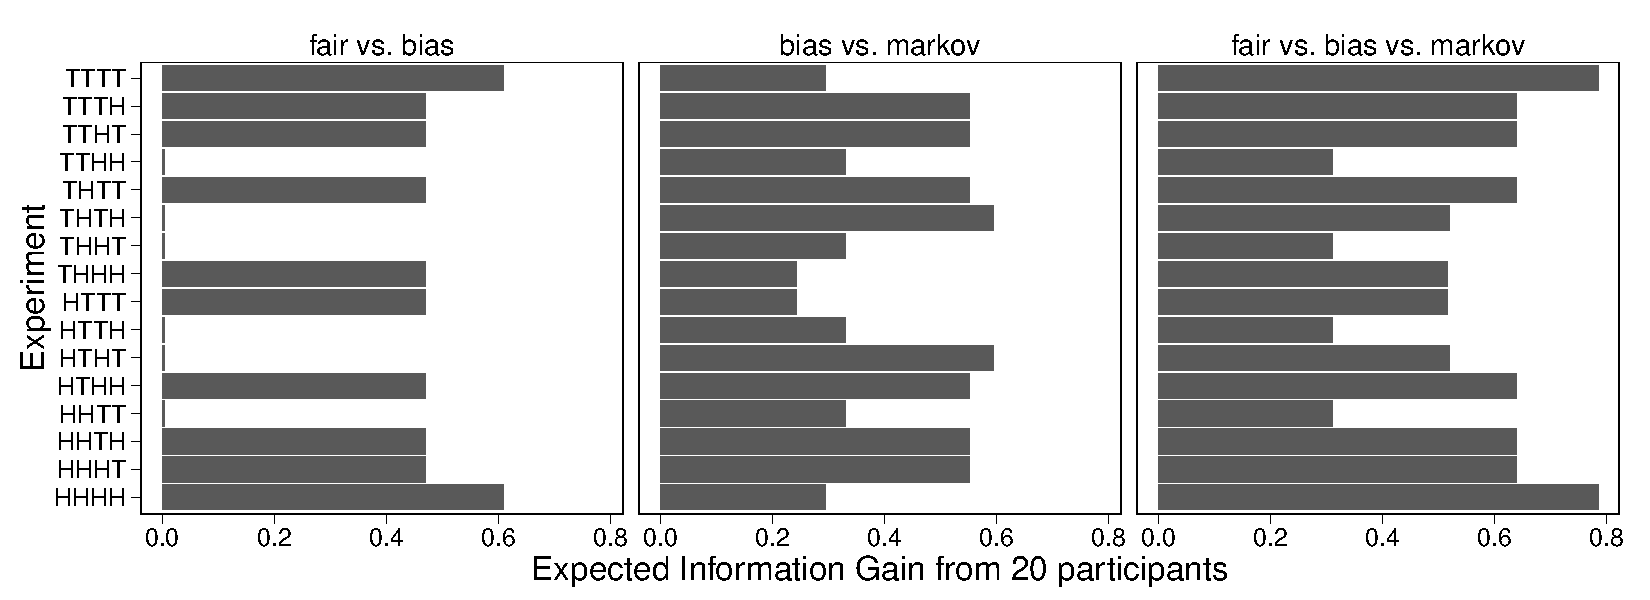
\includegraphics[width=\columnwidth]{img/coin_eig_n20_ignorance.pdf}
\caption{OED call and results for sequence prediction model comparisons with 20 participants.}
\label{fig:run-coin}
\end{figure}
In the example call to \lstinline{OED} (Fig. \ref{fig:run-coin}, Input), we first make composite models using a helper function \lstinline{groupify}, which takes  a function \lstinline{f(x)} and return a function \lstinline{f_group(x,n)}, to reflect predictions for the whole sample of \lstinline{n}.
The experiment space \lstinline{xSample} includes a fixed number of participants and the unique experiments.
The response space \lstinline{ySample} is reflected in an uninformative prior over the number of \lstinline{H} responses (dependent on n).

Consider the fair--bias comparison (Figure \ref{fig:run-coin}, Output, left).
Observe that there are several experiments that have 0 information gain (e.g., \lstinline{HTHT}, see also Figure \ref{fig:coin_preds}a).
This confirms the intuition spelled out before---the models make exactly the same predictions in this case (albeit for different reasons): The experiment has no distinguishing power.
The most informative experiments are \lstinline{HHHH} and \lstinline{TTTT}.
This is also intuitive---the bias model would infer a strongly biased coin and make a strong prediction, while the fair coin model is unaffected by the observed sequence.

Next, consider the bias--Markov comparison.
The least and most informative experiments reverse.
Now, \lstinline{HHHH} and \lstinline{TTTT} are the least informative experiments: Similar to fair--bias comparison, the models make similar predictions for these experiments.
\lstinline{HTHT} and \lstinline{THTH} are the most informative experiments.
This makes sense---the bias model infers a 0.5 probability of heads and so assigns equal probability of heads and tails to the next flip, whereas the Markov model infers that the probability of transitioning is high and assigns high probability to the opposite of whatever outcome was observed last (\lstinline{T} for \lstinline{THTH} and \lstinline{H} for \lstinline{HTHT}).
%Note that the most informative experiments in one model comparison may be the least informative in another.


%\begin{figure}[t]
%\centering
%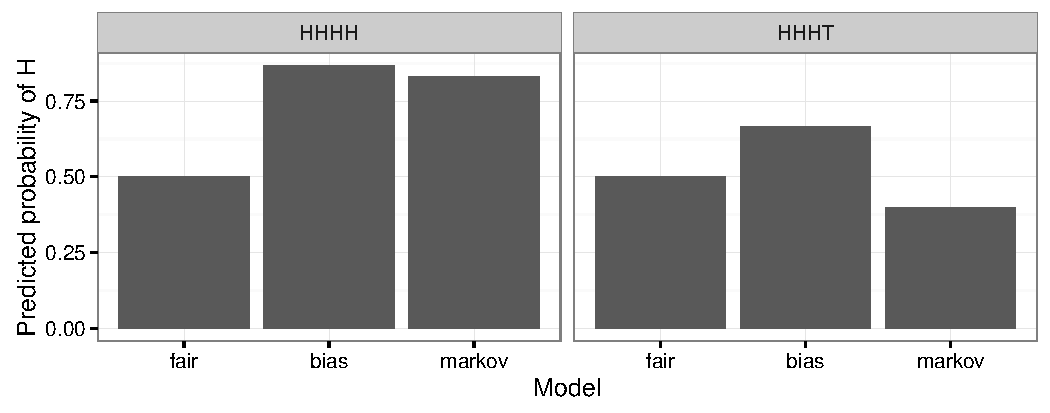
\includegraphics[width=0.7\columnwidth]{img/coin_predictions.pdf}
%\caption{Model predictions for the optimal and penoptimal experiment for distinguishing all three models.}
%\label{fig:coin_preds}
%\end{figure}

\begin{figure}[t]
\centering
\begin{tabular}{l l}
(a) & (b)\\
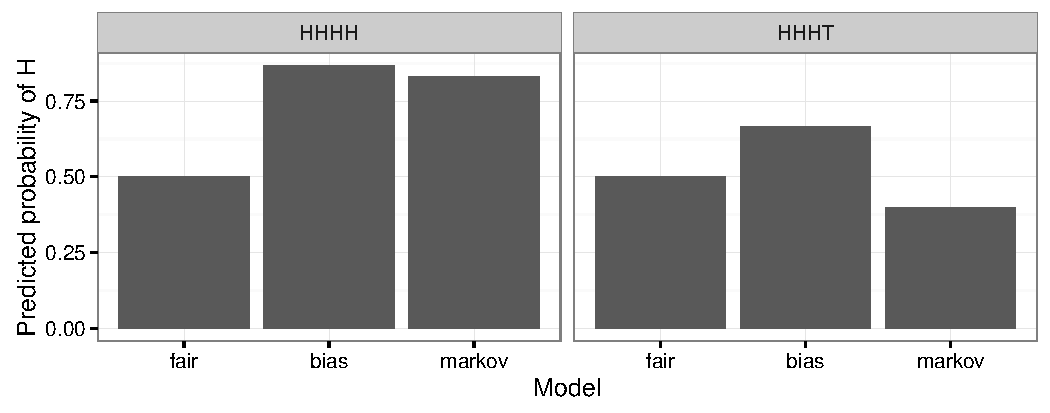
\includegraphics[width=0.6\columnwidth]{img/coin_predictions.pdf} &
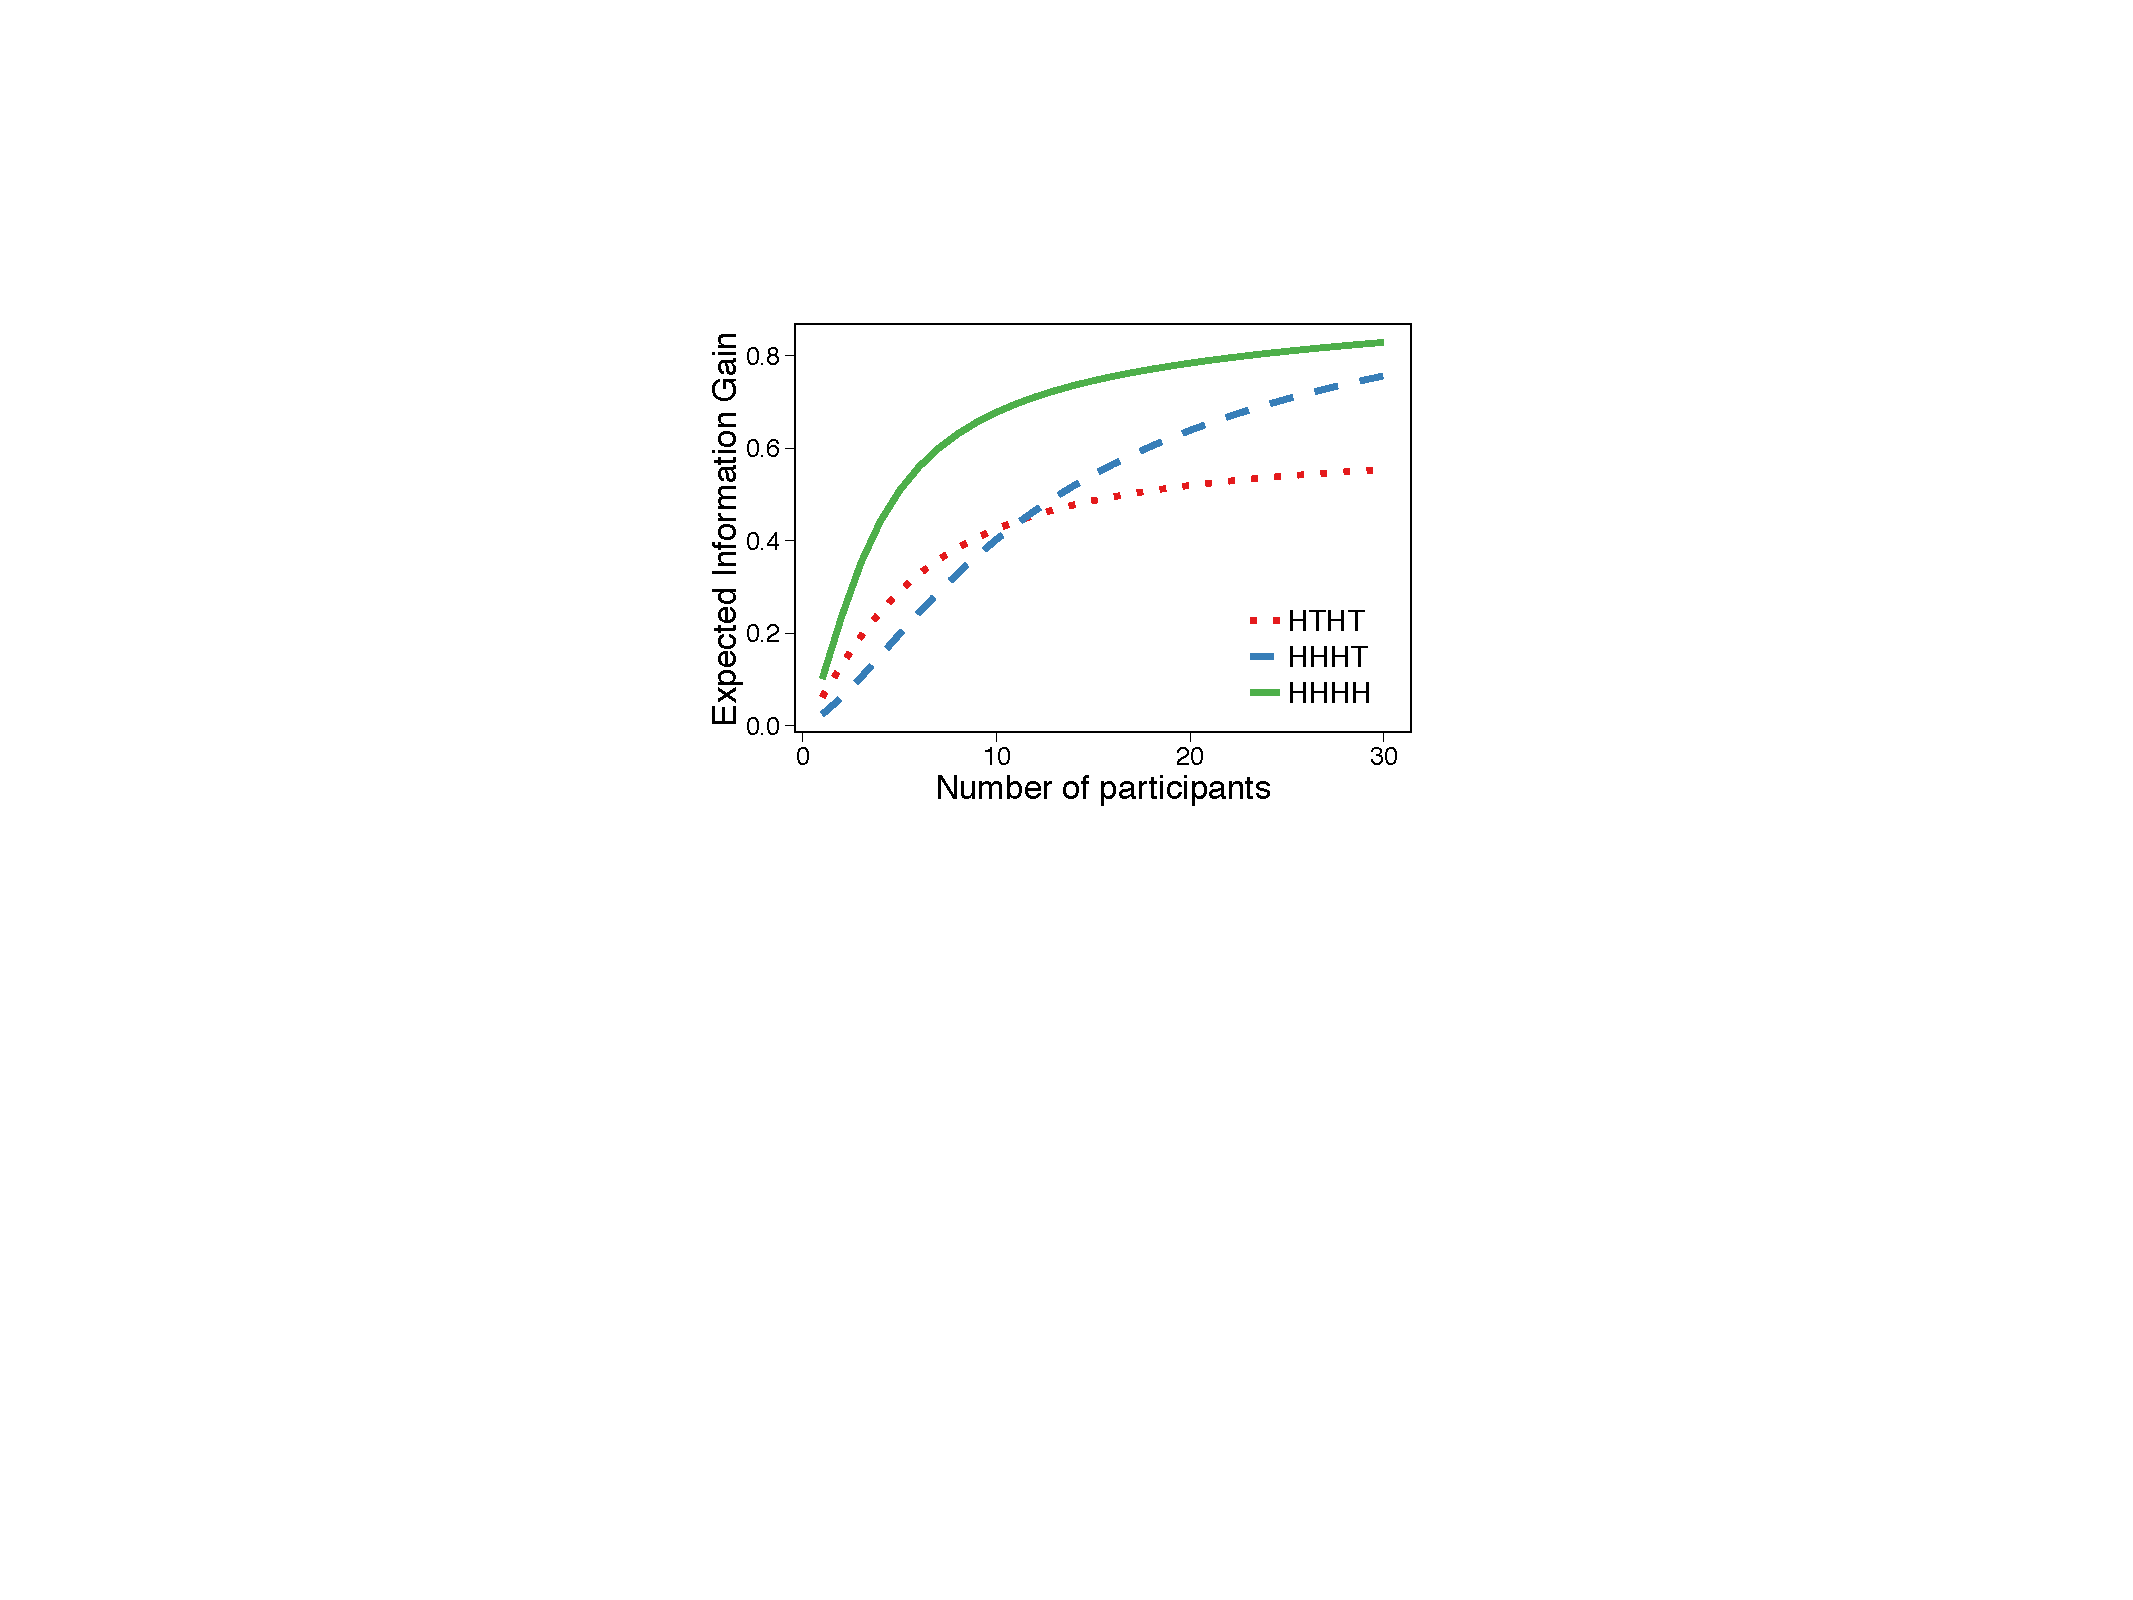
\includegraphics[width=0.4\columnwidth]{img/coin_eig_3way_nsubj_wlegend.pdf} \\\end{tabular}
\caption{(a) Model predictions for the optimal and two other experiments.(b) Expected information gain for distinguishing three models for three experiments as a function of the number of participants.}
\label{fig:coin_preds}
\end{figure}

Finally, consider the fair--bias--Markov comparison.
The worst experiments, \lstinline{TTHH}, \lstinline{THHT}, \lstinline{HTTH}, and \lstinline{HHTT}, are cases where all models make similar predictions.
The best experiments are \lstinline{TTTT} and \lstinline{HHHH}.
The result is non-obvious because we are trying to disambiguate three models.
\lstinline{HHHH} is very good at separating the fair model from the other two models.
The second-most optimal experiment, \lstinline{HHHT}, is much better at distinguishing the bias model from the Markov model (because it predicts a qualitative difference; Figure \ref{fig:coin_preds}a), but the actual information gain is predicted to be less.
An automated tool for experiment design is especially useful in these settings, where human intuition would likely favor the qualitative over the quantitative difference.

The information carried by an experiment will vary according to the number of participants in that experiment.
Figure \ref{fig:coin_preds}b shows the expected information gain in distinguishing the three models for three experiments of interest as a function of the number of participants.
We see the information gain is a non-linear function of the number of participants, and the rank ordering of experiments may change with more participants.
This is particularly relevant when three models are being compared, because small quantitative differences between two models may become more reliable as the sample size grows.
In our example here, the optimal experiment with 1 participant is the same as with 30 participants.


\subsection{Empirical validation}
We validated our OED system by collecting human judgements for all 16 experiments and comparing expected information gain with the actual information gain from the empirical results.
We recruited 351 participants from Amazon's Mechanical Turk and randomly assigned each participant to a single experiment (all of the 16 experiments were completed by $\geq$20 unique participants).
Participants pressed a key to sequentially reveal the sequence of 4 flips and then made a prediction about the of the next coin flip (either heads or tails).
\lou{use consistent level of detail for coin and category experiments}

For each experiment $x$ and result $y$, we computed the expected information gain from running our empirical sample of participants\footnote{N's are $\geq$ 20, because we do client-side randomization. We use the empirical N's for EIG in comparisons to AIG.} and compared this to the actual information gain, $\dkl{P(M \mid Y = y, X = x)}{P(M)}$, for the three model comparison scenarios.
Figure \ref{fig:aig_vs_eig} shows that expected information gain is a reliable predictor of the empirical value of an experiment (minimum $r$ = 0.857). This indicates that the OED tool could be relied on to automatically choose good experiments for this case study.

\begin{figure}[t]
\centering
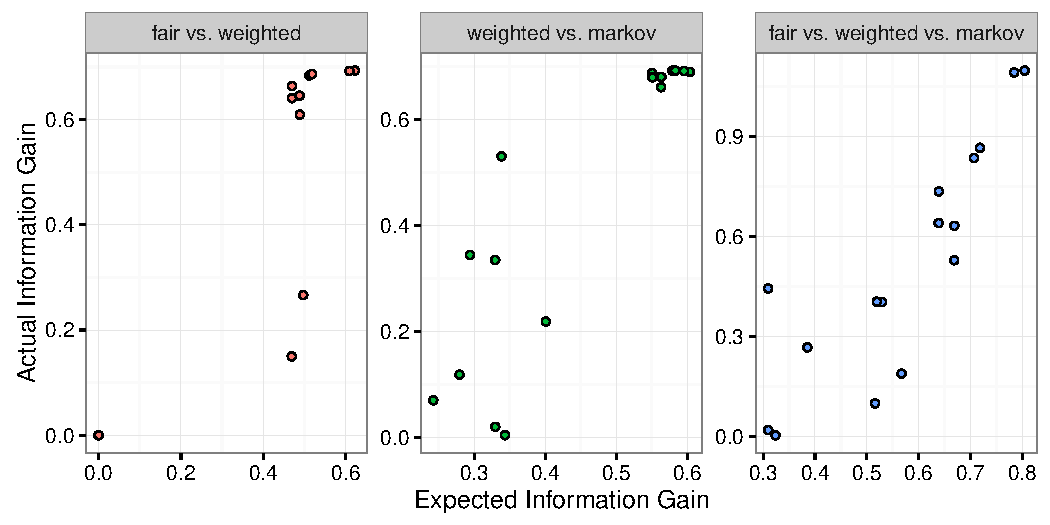
\includegraphics[width=0.7\columnwidth]{img/coin_eig_aig_scatter_noText.pdf}
\caption{Actual vs. Expected Information Gain for each possible experiment, across three model comparison setups.}
\label{fig:aig_vs_eig}
\end{figure}

\section{Case study 2: Category learning}

Here, we explore a more complex and realistic space of models and experiments.
In particular, we analyze a classic paper in the psychology of categorization by Medin and Schaffer \cite{medin78:pr} that aimed to distinguish two competing models of category learning -- the \emph{exemplar model} and the \emph{prototype model}.
Using intuition, Medin and Schaffer (MS) designed an experiment (often referred to as ``the 5-4 experiment'') where the models made diverging predictions and found that the empirical data from this experiment supported the exemplar model.
Subsequently, many other authors followed their lead, replicating and using this experiment to test competing models.
Here, we ask: how good was the MS 5-4 experiment?
Could they have run an experiment that would have distinguished the two models with less data?
%was more information-theoretically efficient?
%Using our OED framework, we find that there are many superior experiments that Medin and Schaffer could have designed but did not.

%\footnote{Our work here is an exercise in counterfactual history; the Medin and Schaffer models are not state of the art. We chose the Medin and Schaffer research (rather than newer work) as an object of study because it commits to a clear set of competing models and a clear set of possible experiments.}



\subsection{Models}

Both the exemplar and prototypes model are classifiers that map inputs (objects represented as a vector of Boolean features) to a probability distribution on the categorization response (a label: A or B).
The exemplar model assumes people store information about every instance of the category they have observed; categorizing an object is thus a function of the object's similarity to all of the examples of category A versus the similarity to all of B's examples.
By contrast, the prototype model assumes that people store a measure of central tendency for each category---a prototype.
Categorization of an object is thus a function of its similarity to the A prototype versus its similarity to the B prototype.
For details, and representation of these models in WebPPL, see the supplement.

\subsection{Experiments}

Participants first learn about the category structures in a training phase where they perform supervised learning of a subset of the objects and are then tested on this learning in a test phase.
During training, participants see a subset of the objects presented one at a time and must label each object.
Initially, they can only guess at the labels, but they receive feedback so that they can eventually learn the category assignments.
After reaching a learning criterion, they complete the test phase, where they label all the objects (training set and the held out test set) without feedback.

MS used visual stimuli that varied on 4 binary dimensions (color: \emph{red} vs. \emph{green}, shape: \emph{triangle} vs. \emph{circle}, size: \emph{small} vs. \emph{large}, and count: \emph{1} vs. \emph{2}).
For technical reasons, they considered only experiments that (1) have linearly separable decision boundaries and (2) contain 5 A's and 4 B's in the training set.
There are, up to permutation, 933 experiments that satisfy these constraints.

\subsection{Predictions of optimal experimental design}

Using the predictive prior for $p(y; x)$, we computed the expected information gain for all 933 experiments and found that the best experiment (for a single participant) had an expected information gain of 0.08 nats, whereas the MS 5-4 experiment had an expected information gain of only 0.03 nats; thus, the optimal experiment is expected to be 2.5 times more informative than the MS experiment.
Indeed, the MS experiment is near the bottom third of all experiments (Figure~\ref{fig:dist}a).

Why is the MS experiment ineffective?
One reason is that Medin and Schaffer prioritized experiments that predict a qualitative categorization difference (i.e., when one model predicts an object is an A  but another predicts it is a B).
The experiment they designed indeed predicts a qualitative difference in one stimulus, but this has a small magnitude and comes at the expense of little information gain from the remaining eight stimuli.
The optimal experiment is better able to quantitatively disambiguate the models by maximizing the information from all the stimuli simultaneously.

\begin{figure}[t]
\centering
\begin{tabular}{l l}
(a) & (b)\\
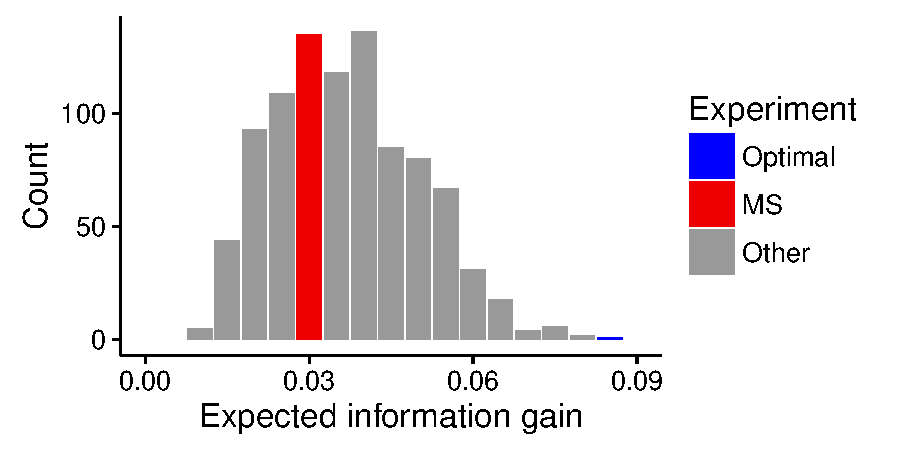
\includegraphics[width=2.5in]{img/category-eig-dist.pdf} & 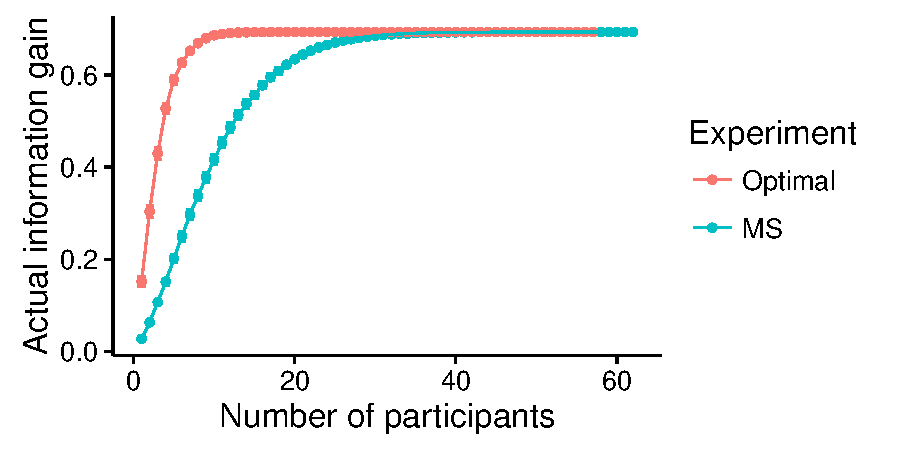
\includegraphics[width=2.5in]{img/category-aig-curve.pdf}\\
\end{tabular}
\caption{(a) Distribution of expected information gain for all possible category learning experiments for a single participant. MS has low expected information gain. (b) Actual information gain versus number of experimental participants included in analysis (error bars are 95\% bootstrapped confidence intervals). MS requires three times as many participants to achieve maximum actual information gain.}
\label{fig:dist}
\end{figure}

\subsection{Empirical validation}

To validate our expected information gain calculations, we ran the MS 5-4 and the optimal experiment with 60 participants each.
Figure~\ref{fig:dist}b shows that the optimal experiment we found for a single participant is indeed better than the MS experiment ($n$=1, blue greater than red).
For $n$=1, the mean AIG for the optimal experiment is 0.15, whereas it is 0.026 for the MS experiment.
This 5-fold difference in informativity is even greater than the 2.5-fold difference we predicted using expected information gain.
In addition, by incrementally introducing more data, we observe both experiments achieve maximal actual information gain but the optimal experiment takes only 10 participants to asymptote to this maximum, whereas the MS experiment takes around 30.
Thus, the optimal experiment provides the same amount of information for a third of the experimental cost.

% and illustrates how automated experiment design can outperform human intuition. In particular, this case study demonstrates the efficacy of OED in psychology for discrete and non-ordinal experiment spaces, large combinatoric experiment spaces, and parametric model classes.

\section{Related work}

The basic intuition behind OED---to find experiments that maximize some expected measure of informativeness---has been independently discovered in a number of fields, including physics \cite{vanDenBerg2003}, chemistry \cite{Huan2010}, biology \cite{Vanlier2012, Liepe2013}, psychology \cite{Myung2009}, statistics \cite{Lindley1956}, and machine learning \cite{Golovin2010}.

These papers, however, implement OED for either one-off or relatively limited cases, specializing for  particular models and committing to a single inference technique.
For example, in systems biology, Liepe et al. \cite{Liepe2013} devised a method for finding experiments that optimize information gain for parameters of biomolecular models (ODEs with Gaussian noise).
Their information measure (Shannon entropy) is similar to ours, but they focus on a narrow family of models and commit to a bespoke inference technique (an ABC scheme based on SMC).
In psychology, Myung \& Pitt \cite{Myung2009} devised a general method but this method requires researchers to select their own utility function for the value of an experiment and implement inference on their own.
For example, they compared six memory retention models using Fisher Information Approximation as a utility function and performed inference using a custom annealed SMC algorithm.
Such ``bring-your-own'' requirements impose a significant burden on practitioners.

By contrast, we show that OED can be expressed as a generic, concise, and flexible function in a probabilistic programming language, which allows practitioners to rapidly explore different spaces of models, experiments, and inference algorithms.
Additionally, our work is the first to (1) demonstrate that expected information gain is a reliable predictor of actual information gain and to (2) characterize the cost benefits of OED.

\section{Conclusion}

Practitioners aim to design experiments that yield informative results.
Our approach partially automates experiment design, searching for experiments that maximally update beliefs about the model distribution.
With our approach, the scientist writes her hypotheses as probabilistic programs, sketches a space of possible experiments, and hands these to OED for experiment selection.
We stress that our work \emph{complements} practitioners; it does not replace them.
Our tool eliminates the need to manually comb large spaces in search of good experiments; we hope this will free scientists and engineers to work on the more interesting problems---devising empirical paradigms and building models.

Our approach suggests a number of interesting directions for future work.
%First, we chose KL divergence between posterior and prior as our informativeness measure because it is a well-known divergence function, but other choices (e.g., TV distance) might also be suitable.
We cast the OED problem as a problem of inference, and this might suggest particular inference techniques.
For instance, if a particular response is quite unlikely (i.e., $p(y)$ is negligible), it may be acceptable to have a less precise estimate of information gain for that response.
Additionally, our framework naturally integrates the cost of experiments into the design computation (as a prior on experiments).
This enables principled treatment of multi-objective optimization problems (e.g., MRI studies of rare patient populations, expensive aerospace experiments).
Finally, we have explored the trajectory of information gain as the number of \emph{i.i.d.} observations increases.
Observations need not independent, however.
Adaptive testing can be formulated as a problem of information gain of sequences of experiments, which produce dependent and non-identical responses.
%Third, we have restricted attention to ``one-shot'' experiments, but it would be interesting to extend our work to sequential settings (e.g., adaptive tests).
%Fourth, we have ignored the cost of experiments, but it would be worth explicitly taking this into account.
%Our informativeness approach could be usefully integrated with for real-world applications (e.g., MRI studies of rare patient populations, expensive aerospace experiments).
In this paper, we showed case studies of our method in cognitive psychology but we believe that it is broadly useful, so we invite practitioners to test our method.

\bibliographystyle{ieeetr}
\bibliography{oed_nips_2016}

\end{document}
